\documentclass[french]{article}
\usepackage[T1]{fontenc}
\usepackage[utf8]{inputenc}
\usepackage{lipsum}
\usepackage{lmodern}
\usepackage{geometry}
\usepackage{babel}
\usepackage{graphicx}
\usepackage{lastpage}
\usepackage{ragged2e}
\usepackage{enumitem}
\usepackage[normalem]{ulem}
\usepackage{hyperref} % pour \url{URL}
\usepackage{color} % pour \textcolor{color}{text}
\usepackage{listings} % pour afficher du code
\usepackage{longtable} % pour l'environnement longtable
\usepackage{float} % pour des figures non flottantes
\usepackage{amsmath}
\usepackage{caption} % figure et subfigure pour mettre les images côtes à côtes
\usepackage{subcaption}
\usepackage{dirtree}
\usepackage{menukeys}

\graphicspath{ {../presentation/uml/img/png/} }

% Style Java
\lstset{
	language=Java,
	tabsize=2,
	basicstyle=\small\ttfamily,
	keywordstyle=\color{blue},
	stringstyle=\color{red},
	commentstyle=\color{black!40},
	morecomment=[l][\color{black!50}]{\#},
	gobble=10,
	frame=single,
	otherkeywords={}
}

\geometry{
	a4paper,
	total={210mm,297mm},
	left=20mm,
	right=20mm,
	top=25mm,
	bottom=25mm,
}

\usepackage{fancyhdr}
\pagestyle{fancy}
\setlist[enumerate,1]{leftmargin=2cm}

% Entêtes
\lhead{Browne, Champion, Clément, Hardy}
\chead{}
\rhead{MCR: Rapport}
\renewcommand{\headrulewidth}{0.4pt}
\renewcommand{\footrulewidth}{0.4pt}

\begin{document}
	
	% Titre du document
	\title{Sokonet}
	\author{Rapport\\ 
		Projet de MCR\\
		Browne Champion Clément Hardy\\
		Resp. Pier Donini\\
		HEIG-VD}
	\date{\today} % date du jour
	\maketitle
	\centering
	$ $\newline
	$ $\newline
	$ $\newline
	$ $\newline
	$ $\newline
	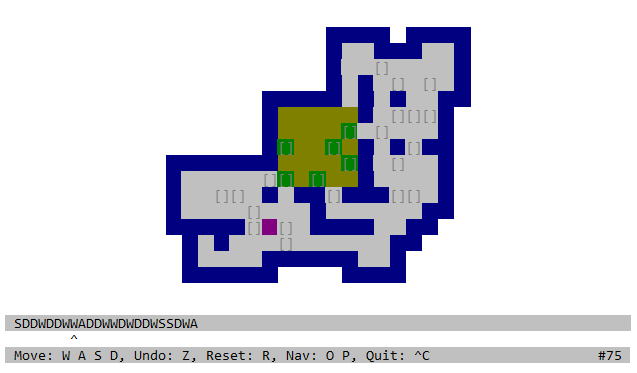
\includegraphics[scale=0.8]{titre}
	\thispagestyle{empty}
	
	\newpage
	\thispagestyle{empty}
	$ $
	\newpage
	
	% Pour tout le document
	\justify
	\normalsize
	
	% Tables des matières
	%\tableofcontents
	%\newpage
	
	\section{Introduction}
	Suite à la présentation théorique dans le cadre du cours de MCR, il nous a fallu réaliser une application sur la base d'un modèle. Celui nous ayant été attribué est le modèle de conception "commande". Dans l'idée d'utiliser au mieux les possibilités proposées par le modèle, c'est-à-dire l'annulation de commande et l'utilisation de macros, il nous est venu l'idée d'implémenter le \textit{Sokoban}. Ce dernier tournant sur un serveur et accessible depuis un terminal telnet, d'où le nom de \textit{Sokonet}.
		
	\section{Contexte de mise en œuvre}
	Le Sokoban est un jeu de puzzle dont le but est de pousser des caisses jusqu'à un lieu donné. Il s'agit d'un jeu en deux dimensions dont les déplacements se font de case en case. De par la nature du jeu, il est possible de se bloquer dans la réalisation d'énigme. Par exemple, une caisse se situant dans un coin, ne peut plus être déplacé. À moins que ce coin ne soit une destination à atteindre, le joueur se retrouvera complètement bloqué par l'impossibilité de pouvoir déplacer la caisse jusqu'au bon endroit. Le modèle de conception "commande" permet alors de se sortir de telles situations. En effet, si tous les mouvements de l'utilisateur sont stockés dans un historique, il est possible d'annuler chaque mouvement et ses effets dans le jeu. Le modèle de conception autorise également l'utilisation de macros, soit une combinaison de plusieurs commandes.
	
	\section{Diagramme de classe}
	\begin{figure}[H]
		\centering
		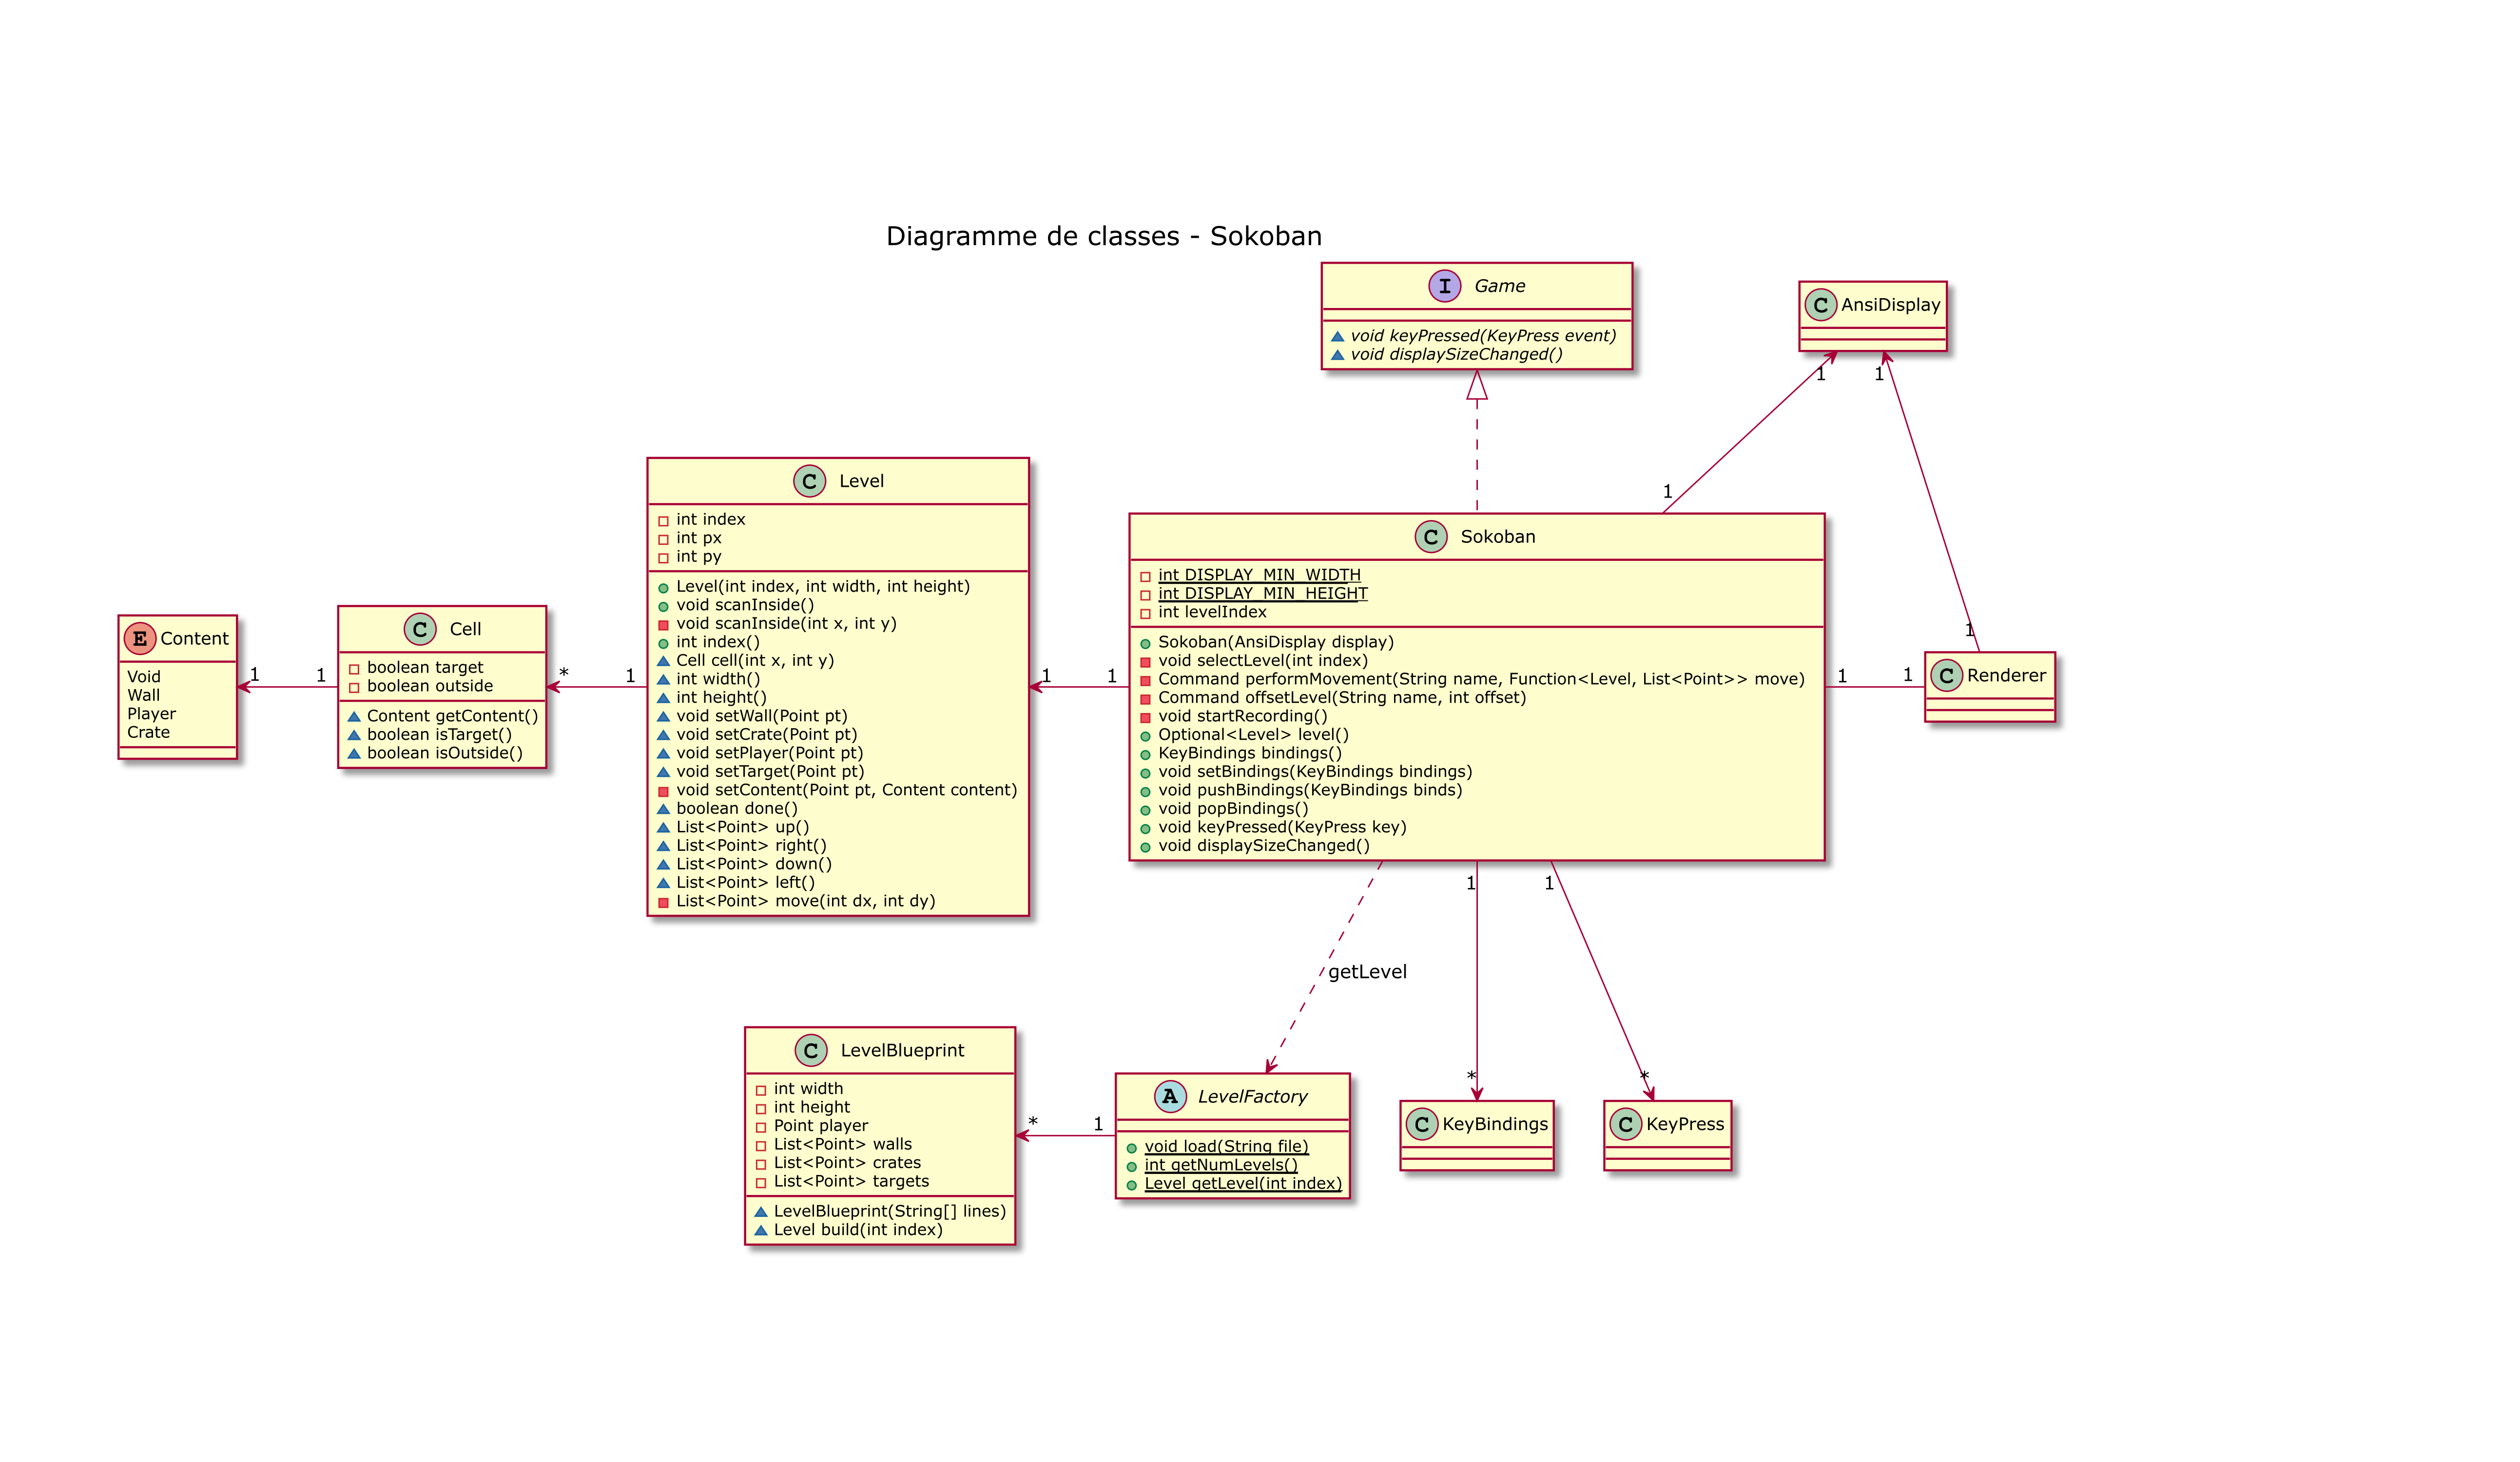
\includegraphics[width=\textwidth]{sokoban}
		\caption{Diagramme de classes principal}
		\label{classDiagMain}
	\end{figure}
	
	\begin{figure}[H]
		\centering
		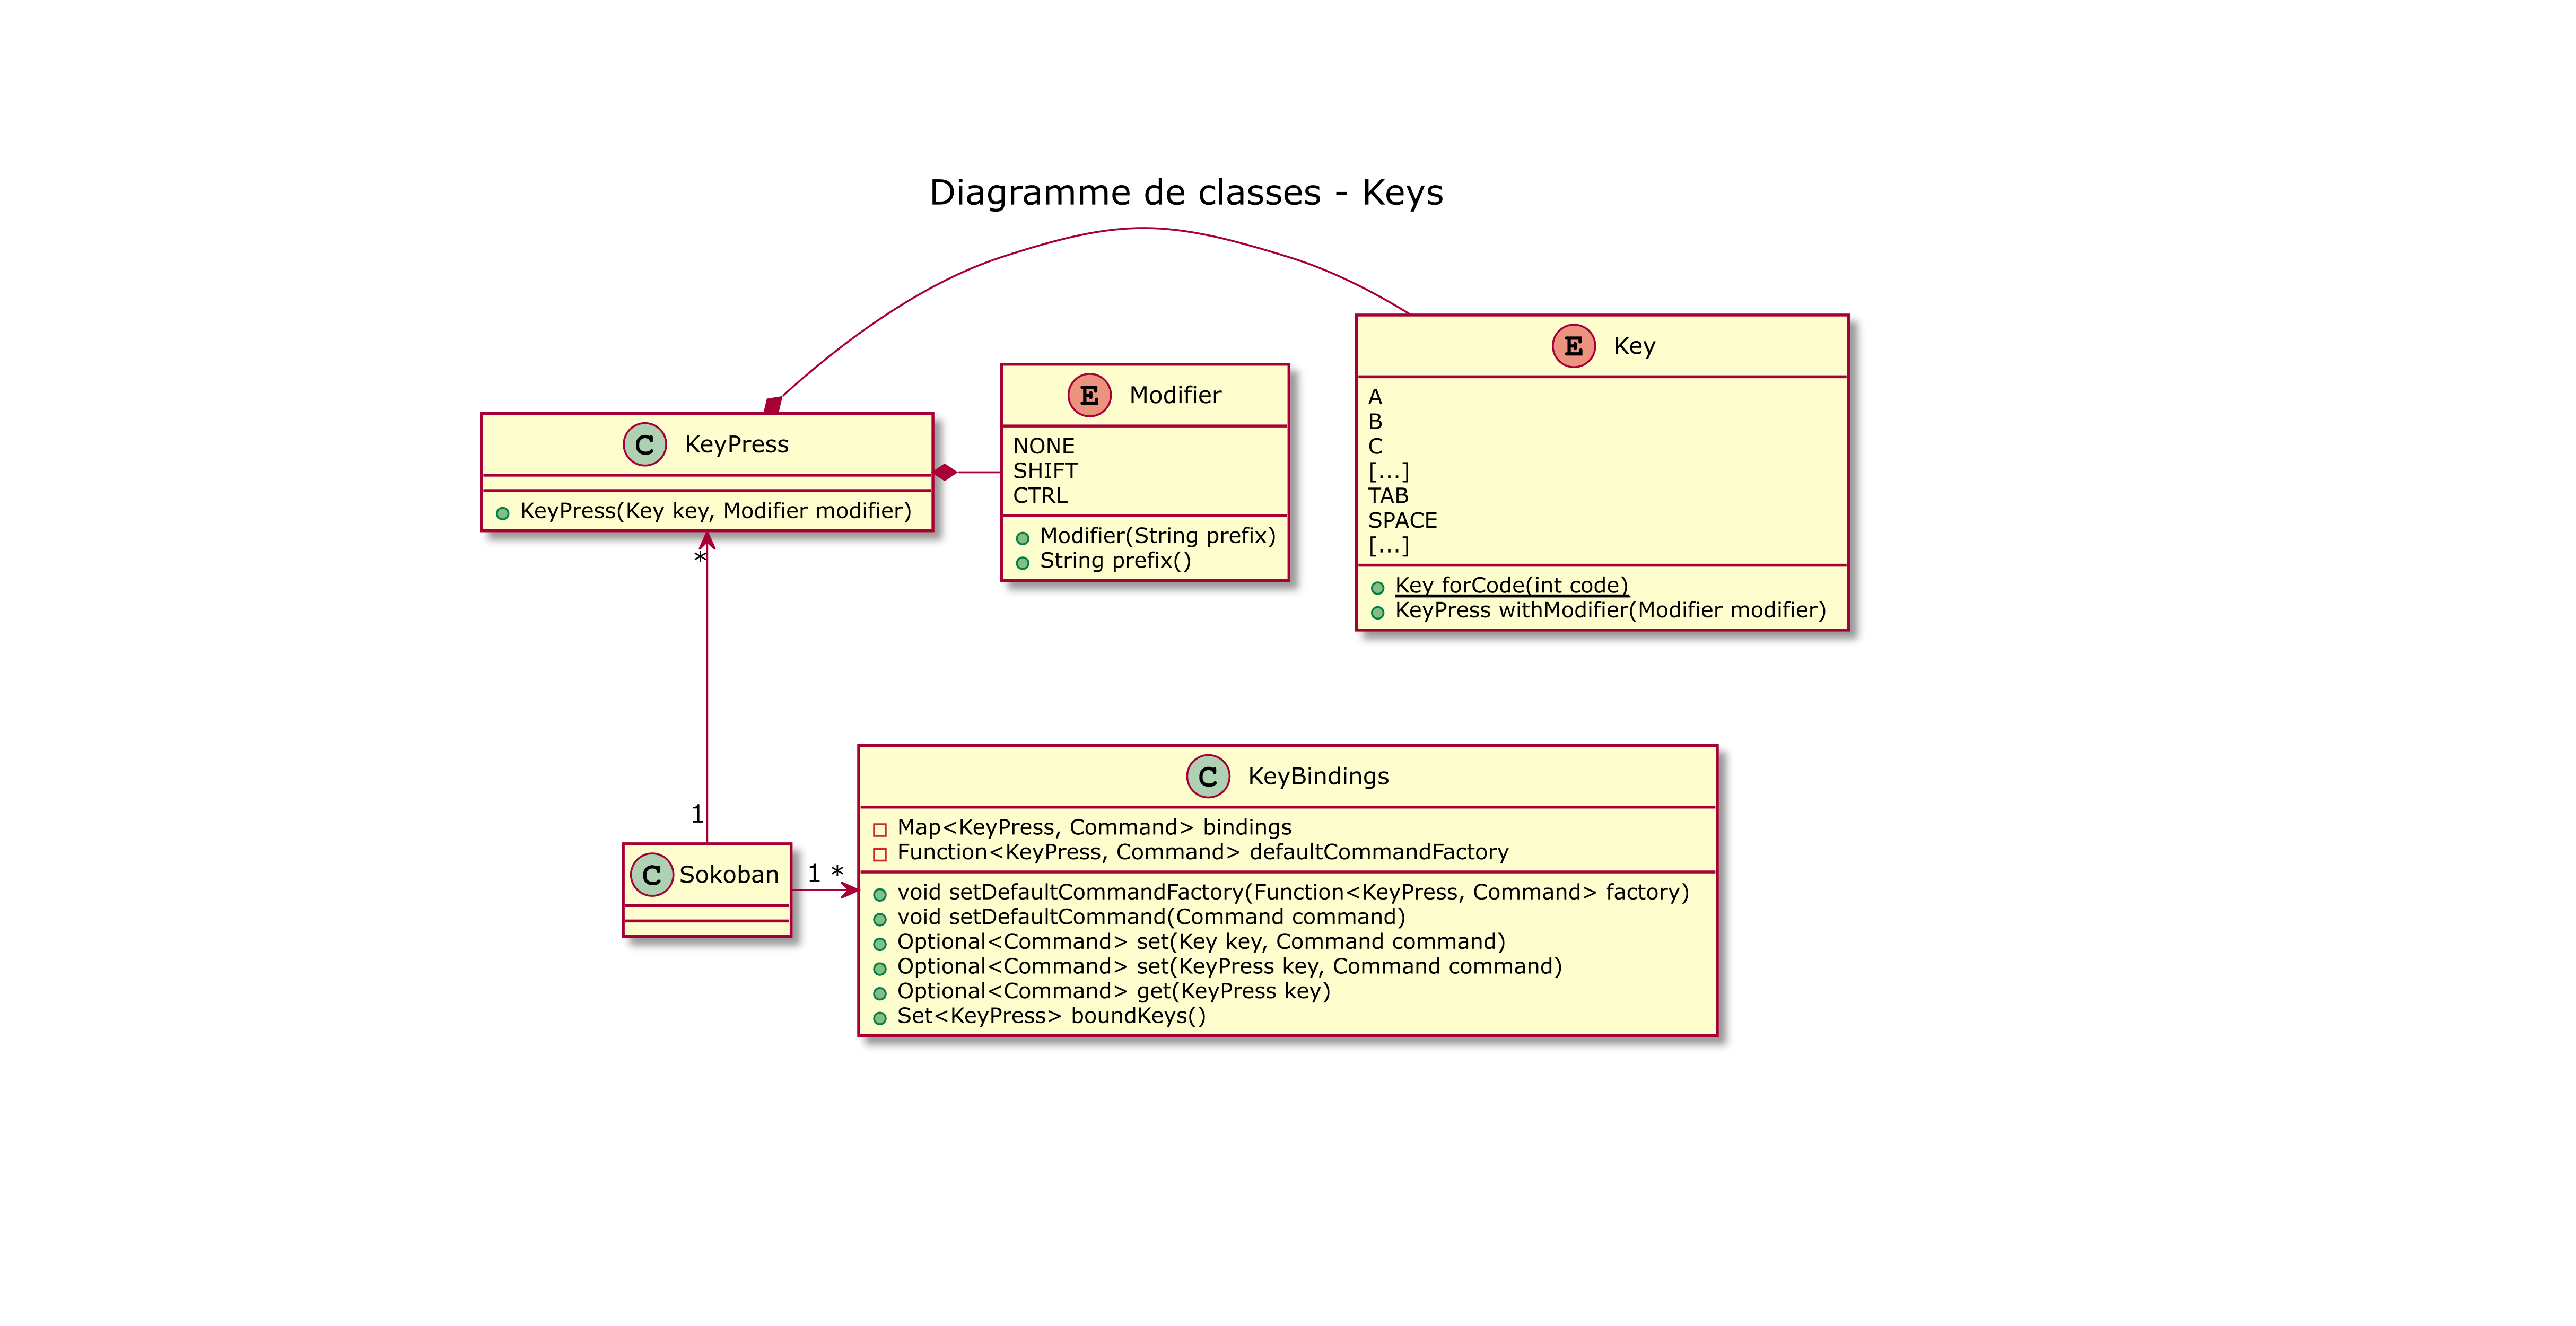
\includegraphics[width=0.8\textwidth]{keys}
		\caption{Diagramme de classes pour la gestion des touches}
		\label{classDiagKey}
	\end{figure}
	
	\begin{figure}[H]
		\centering
		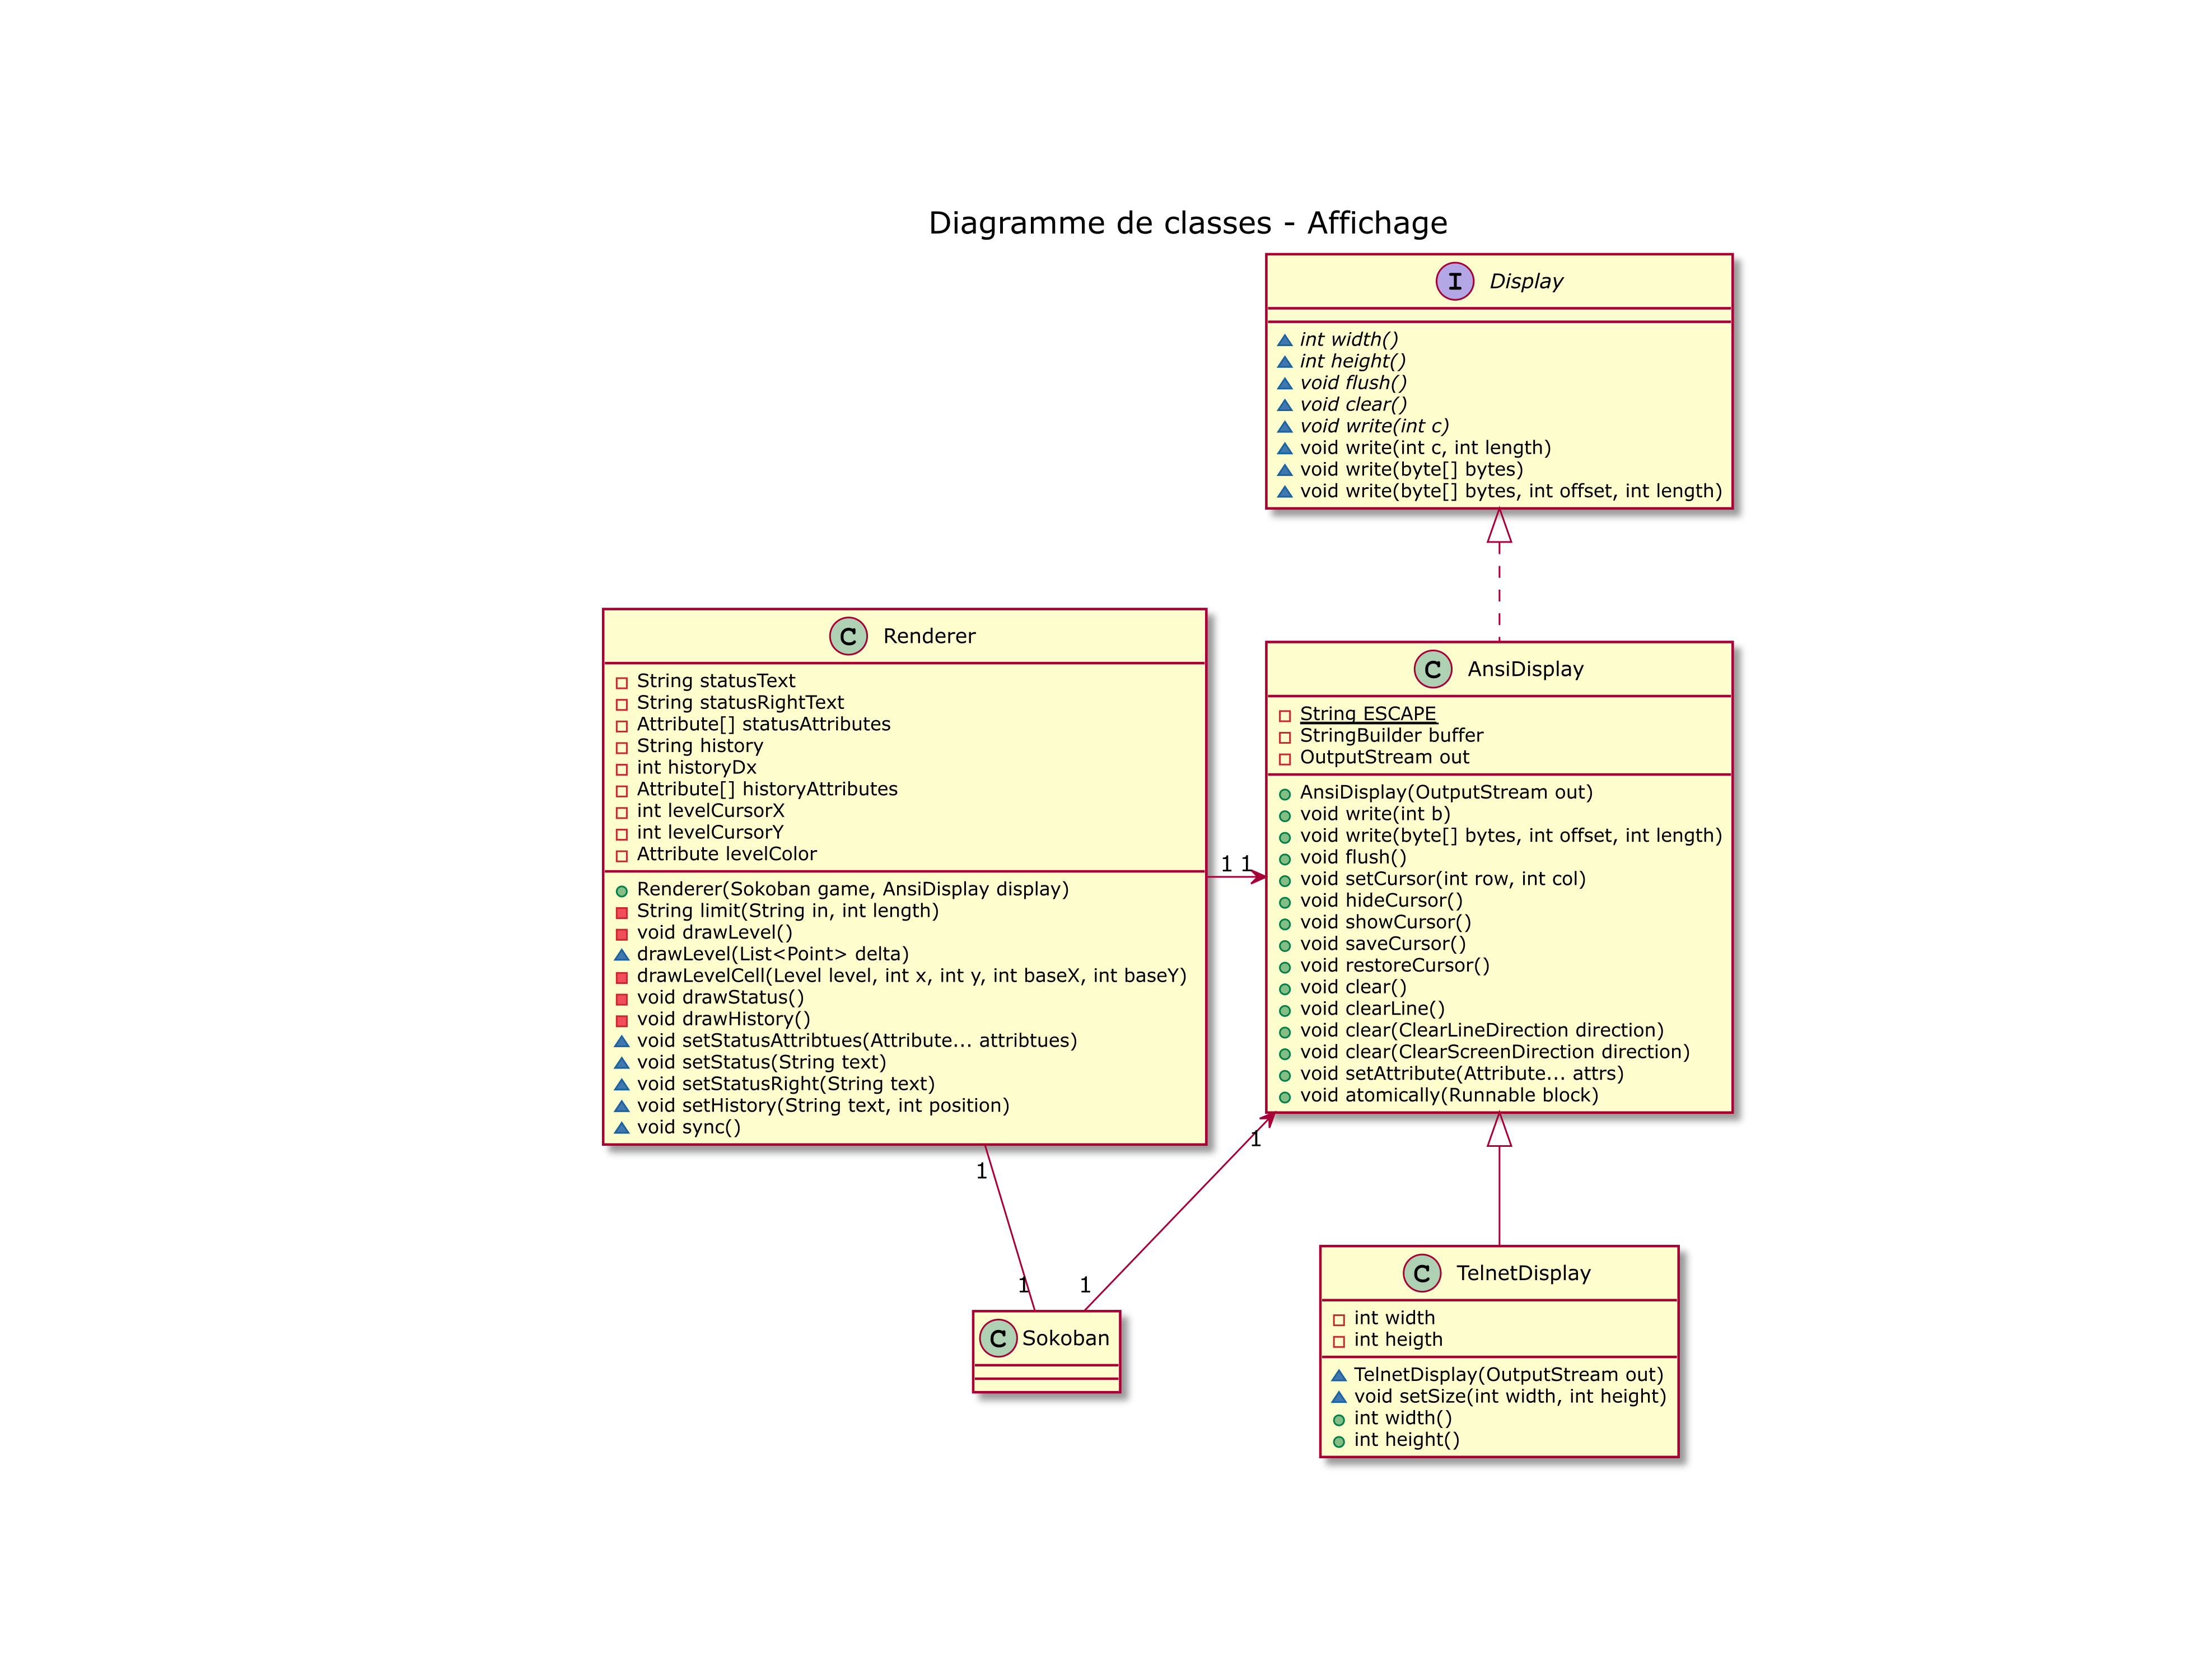
\includegraphics[width=0.8\textwidth]{affichage}
		\caption{Diagramme de classes pour la gestion de l'affichage}
		\label{classDiagDisplay}
	\end{figure}
	
	Le diagramme de classes a été décomposé en trois parties: en \textbf{figure \ref{classDiagMain}} la partie principale qui gère la logique du jeu, puis la partie de gestion des touches en \textbf{figure \ref{classDiagKey}} et enfin les classes qui s'occupent de l'affichage en \textbf{figure \ref{classDiagDisplay}}. Sous sa forme actuelle, l'implémentation du \textit{command pattern} permet le \textit{rollback} des déplacements de l'utilisateur et des caisses si nécessaire avec la touche \keys{Z}. Il est également possible d'enregistrer des macros en appuyant sur la touche \keys{M}, puis les mouvements souhaités et \keys{M} à nouveau, avant de l'assigner à une nouvelle touche.
	
	\section{Conclusion}
	Ce travail pratique nous a permis d'apprendre et de comprendre un modèle de conception que nous n'avions pas vu en cours mais qui se révèle fort pratique. Ce modèle est souvent utilisé quand il s'agit de faire un historique de commandes et de pouvoir les annuler. Grâce à cela, nous avons dû l'apprendre et le comprendre, afin de pouvoir le présenter. La création d'un serveur telnet a permis d'en apprendre également plus sur cette technologie et son fonctionnement, notamment pour la gestion de l'affichage. Nous avions certes implémenté un petit exemple pour la présentation théorique du modèle, mais avoir implémenté dans une véritable application le modèle nous a aidé à mieux comprendre le fonctionnement derrière cette façon de concevoir des programmes.
\end{document}
